\hyperref[sec:sec25]{\section{為什麼香港的法院會有外籍法官?}}
\label{sec:sec24}

因為《基本法》草擬的時候,中國政府有自知之明,理解到保證司法制度健全才能讓香港和國際社會對九七後的管治保持信心,否則即使收回香港也只會成為中國的負擔而不能有所貢獻。香港的法院有外籍法官,正是當時這點擔憂的體現。按照《基本法》,除了終審法院和高等法院的首席法官應由在外國無居留權的香港特別行政區永久性居民中的中國公民擔任外,香港的法官沒有國籍限制。

香港法院外籍法官的法理依據,來自《基本法》第八十二條:「終審法院可根據需要邀請其他普通法適用地區的法官參加審判」和第九十二條:「香港特別行政區的法官和其他司法人員,應根據其本人的司法和專業才能選用,並可從其他普通法適用地區聘用」。現時香港終審法院有一名首席法官、三名常任法官、四名香港非常任法官,以及十二名海外非常任法官。

這些條文的來源要算到八十年代初,《中英聯合聲明》尚未訂立之時,中國政府對香港前途的考量。這時期的香港各界人心惶惶,畢竟中國大陸才剛剛脫離文革浩劫,擔心中國收回香港就是香港終結之時。對於法律界來說,他們看到香港執行的是普通法制度,和中國大陸執行的社會主義法制並不相容。舉個例,香港從開埠以來就是一個自由港,相對公平和有效率的司法制度讓商人有信心任合何糾紛都可以得到合理的訟裁。如果法官容易受一時的政治壓力或貪污收買所影響,商人就要面對一個隨意和不可靠的環境,做生意的成本就會大幅增加。當時的中國正處於改革開放的早期,需要通過香港吸引外來投資。如果外資都從香港撤走,那麼不單止香港本身的繁榮穩定不能維持,連帶中國大陸的發展也會受到阻礙。

因此,當時的中國政府注意到香港社會的憂慮,並於一九八三年邀請了十二位本地年輕專業人士到北京訪問,並和時任中共中央書記處書記習仲勛見面(也就是現任國家主席習近平的父親)。這個「才俊團」的成員很多後來都成為香港政界翹楚,例如特區首任終審法院首席法官李國能等。而據另一位成員李柱銘回憶所述,這段時間的中港交流對日後特區的制度框架起了重要作用。

李柱銘是民主黨創黨主席,被中國政府視為反對派,但這其實是八九民運之後的事。他是香港排名首位的資深大律師(九七前稱御用大律師),在香港的法律界有極為顯赫的地位,因而也曾被中國政府視為拉攏對象,並在一九八五年被委任為《基本法》起草委員會的成員。不過到了北京六四鎮壓後,他便毅然退出,從此與中共決裂。

回到八十年代初,當「才俊團」回到香港後,成員聚餐回謝新華社(當時中國政府的駐港代表)的聯繫。按李柱銘的回憶所述,席間他與時任副社長的李菊生提到終審法院的問題。九七前香港的法庭申訴最終可送往英國倫敦樞密院,李柱銘向李菊生提到要保持香港在九七後的穩定,司法制度要給予外國投資者信心,讓他們相信日後在香港遇到任何法律問題,法庭也會如樞密院的法官一樣中立公正。李菊生同意中國的司法制度不能做到這點,便請李柱銘提意見。於是李柱銘便提議把終審法院設在香港,用香港的律師,按香港的案例判案。他更進一步提議部份終審法院的大法官可由其他普通法地區邀請過來,而李菊生也認為是好主意。後來《中英聯合聲明》頒佈,容許任命外籍法官的規定在附件一第三部當中列明,再後來成為上面列出的《基本法》第八十二條和第九十二條。

這段歷史說明中國政府的對港政策從來都要考慮外界的反應。香港作為一個特區的地位不是純綷中國政府自己說了算,不是中國政府說香港是一個特區,世界各地就自然會把香港視之為一個特區看待。世界各地必須要看到香港有各種制度保證香港的獨特性,而且這些制度有效運行,才會承認香港的特區地位,並予以相關的待遇,例如商貿往來的各種政策(見問題十七)。外籍法官的制度設計正正是為了回應外界地一國兩制的疑慮。

香港的法院有外籍法官這回事,在特區成立以來的爭議一直不大,要到了近年才被一些中國政府負責香港事務的官員、香港的建制陣營,以及一些內地輿論所質疑。近年多宗與二零一四年佔領運動相關的官司判決,每當出現抗爭者勝訴,又或執法者被判濫權,便會有內地傳媒輿論連帶質疑外籍法官制度,聲稱國籍效忠的問題會影響到他們的判斷。這種質疑其實不難理解,畢竟在官方審查之下是不可能承認這些不符合其政治立場的判決的公正性,法官的國籍成為一個方便的推卸藉口,判詞中提到的各種司法理據便可以被略去不提了。《人民日報》和《環球時報》就為此發表了多篇評論文章,基本法委員會委員饒戈平也曾聲稱香港有外籍法官只是過渡安排,日後可考慮修改。

這些說法在香港社會引來不少憂慮。畢竟,香港本身對於法官的委任已有多年行之有效的制度,一直只看其專業能力而不論出身背景。外籍法官的議論,背後假定了外籍法官判案時沒有或拒絕考慮到一些中國籍法官才會考慮的因素,並視之為一種缺失,其實已是對香港司法制度的蔑視。此外,《基本法》第九十二條例明法官「應根據其本人的司法和專業才能選用」,並沒有政治立場審查的前設,所以整個法官國籍的討論本來就不符合《基本法》訂明的原則。

外籍法官的爭議並非單獨事件。國務院於二零一四年發表的《「一國兩制」在香港特別行政區的實踐》白皮書,就把「各級法院法官和其他司法人員等」定義為「治港者」,所以有維護國家主權、安全、發展利益的職任,而「愛國是對治港者主體的基本政治要求」。此等理解,明顯和容許外籍法官的制度本身矛盾,也完全違背了香港社會一直以來對司法制度的理解。香港社會對法治的追求向來強調「以法限權」,即法律可限制管治者如何行事,公權力受法律約束;而非僅僅「有法可依」和「有法必依」,即管治者通過法律來行事,說到底政府仍然高於法律。然而「白皮書」的說法,卻明顯地是基於後者,僅僅視司法制度為管治的工具而非前設。

\begin{figure}[htbp]
    \centering
    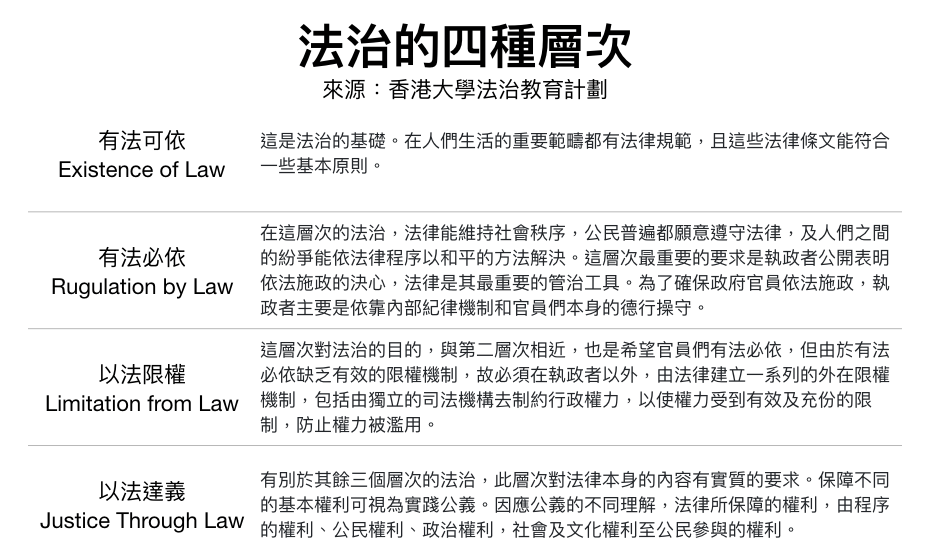
\includegraphics[width=0.7\textwidth]{c24/h-klesson1-040.png}
    \caption{法治的四個層次(香港大學法律學院)} 
\end{figure}

總的來說,外籍法官爭議的意義並不限於這些法官本身,而是如何理解司法制度的運作和價值。如果判決不合乎某一方的政治訴求,要在法理上辯論和反省固然無可厚非。但把矛頭指在外籍法官之上,認為他們先驗地有所偏差,本身就是對司法制度的運作和價值有所誤解。

最後,得再重申一次香港是個國際城市,香港永久性居民不一定是中華人民共和國公民(見問題十一)。《基本法》在制度上已清晰列明,除了少數最高級別的職位外,不一定要中華人民共和國公民才可出任公職。除了法官之外,《基本法》第六十七條列明立法會可有不多於五分之一的非中國籍或持外國居留權的議員。此外,第九十九條和第一百零一條又列明公務人員不一定要是中國國籍,只有廉政專員、審計署署長、警務處處長、入境事務處處長和海關關長例外。即使是《基本法》第一百零四條的就職宣誓要求,也只限於「效忠中華人民共和國香港特別行政區」,而非「效忠中華人民共和國」本身。既然香港政府可以有外籍公務員,香港立法會可以有外籍議員,那麼香港的司法機構有外籍法官其實應不足為奇。



伸延閱讀:

馬嶽(2012):〈李柱銘:他也曾經「親中」〉,《香港80年代民主運動口述歷史》,香港:香港城市大學出版社。

Ghai Y(1999) The Legal and Judicial System, \textit{Hong Kong's new constitutional order: the resumption of Chinese sovereignty and the Basic Law}. Hong Kong: Hong Kong University Press.

網上資源:

\href{http://www.role.hku.hk/levels}{香港大學法律學院(2017)法治層次:法治教育計劃,2017年}

\href{https://www.inmediahk.net/node/1056029}{法夢(2018)與《香港01》商榷︰評海外法官任命不宜借題發揮:香港獨立媒體網,2018年3月28日}